\documentclass[12pt, a4paper]{article}
\setlength{\parindent}{0pt}
\usepackage{amsmath}
\usepackage{amsthm}
\usepackage{amssymb}
\usepackage{graphicx}
\usepackage[a4paper, portrait, margin=1in]{geometry}

% i like the black square better.
\renewcommand{\qedsymbol}{$\blacksquare$}
%\renewcommand{\implies}{\Rightarrow}

\newcommand{\N}{\mathbb{N}}
\newcommand{\ddx}{\frac{d}{dx}}
\newcommand{\Ddx}[2]{\frac{d#1}{d#2}}

\newtheorem{theorem}{Theorem}

% let's begin
\begin{document}
\textbf{(Q1)}

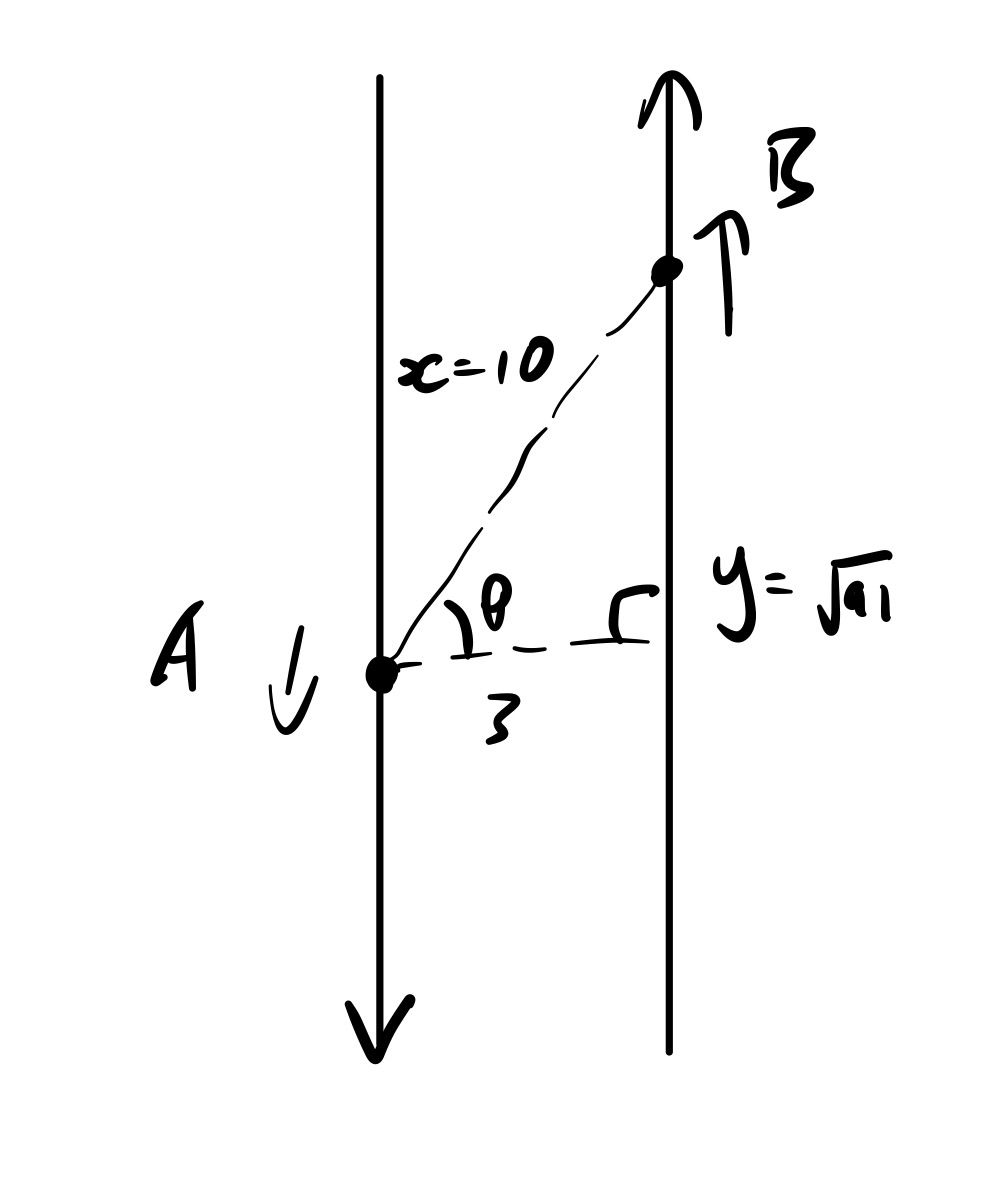
\includegraphics[width=7cm]{related_rates.jpg}

We complete this problem from car A's perspective. From that perspective, car B
is travelling north at 130km/h. Thus, $\Ddx{y}{t} = 130$. We want $\Ddx{x}{t}$.

By Pythagoras' Theorem, we have $x^2 = y^2 + 9$. Differentiating both sides,
we have
\[
    2x \cdot \Ddx{x}{t} = 2y \cdot \Ddx{y}{t}
    \implies \Ddx{x}{t} = \frac{2y \cdot \Ddx{y}{t}}{2x}
\]

Since we know $x = 10$, by Pythagoras' Theorem:

\[
    100 = y^2 - 9 \implies y^2 = 91 \implies y = \sqrt{91}
\]

Then,

\[
    \Ddx{x}{t} = \frac{2\sqrt{91} \cdot 130}{20} = 13\sqrt{91}
\]

Thus, the rate of change of the distance between them is $13\sqrt{91}$ km/h.

\end{document}